\documentclass{article}
% translate with >> pdflatex -shell-escape <file>

% This file is an extract of the PGFPLOTS manual, copyright by Christian Feuersaenger.
% 
% Feel free to use it as long as you cite the pgfplots manual properly.
%
% See
%   http://pgfplots.sourceforge.net/pgfplots.pdf
% for the complete manual.
%
% Any required input files (for <plot table> or <plot file> or the table package) can be downloaded
% at
% http://www.ctan.org/tex-archive/graphics/pgf/contrib/pgfplots/doc/latex/
% and
% http://www.ctan.org/tex-archive/graphics/pgf/contrib/pgfplots/doc/latex/plotdata/

\usepackage{pgfplots}
\pgfplotsset{compat=newest}

\pagestyle{empty}

\begin{document}
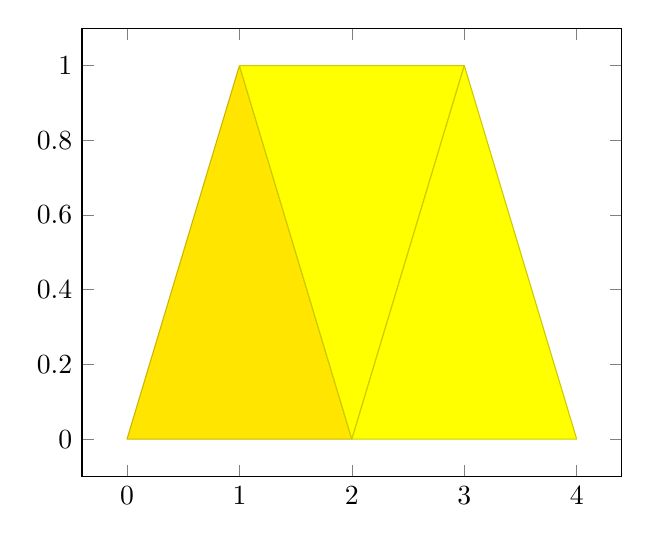
\begin{tikzpicture}
	\begin{axis}
	\addplot[patch,table/row sep=\\,patch table={%
		0 1 2\\
		1 2 3\\
		4 3 5\\
	}]
	table[row sep=\\,point meta=\thisrow{c}] {
		x y c  \\
		0 0 0.2\\% 0
		1 1 0  \\% 1
		2 0 1  \\% 2
		3 1 0  \\% 3
		2 0 0.5\\% 4
		4 0 0.5\\% 5
	};
	\end{axis}
\end{tikzpicture}
\end{document}
